% =============================================================================
\chapter{Comparison with an exact method}
\label{cha:exact}
% =============================================================================

The first test for an approximate theory is usually a comparison with exact analytical predictions, when it is possible.
For systems where the functional truncated Wigner method really shines~--- the ones with hundreds of thousands of particles and thousands of modes~--- no exact methods exist.
However, one can perform such a comparison for the multimode truncated Wigner with only a few modes.
While it does not demonstrate the full extent of the truncated Wigner's functionality, it can still give a general idea about the accuracy of the method.
In this chapter we will investigate a simple two-level system, the dynamics of which can be described exactly using an expansion in number states, and simulate its evolution using the Wigner representation.


% =============================================================================
\section{Two-mode BEC example}
% =============================================================================

We consider a single-well two-mode \abbrev{bec} system with the Hamiltonian
\begin{eqn}
    \hat{H} / \hbar
    = \frac{1}{2} \sum_{i,j=1}^2 g_{jk}
        \hat{a}_j^\dagger \hat{a}_k^\dagger \hat{a}_k \hat{a}_j,
\end{eqn}
which is a special case of the two-well four-mode system described elsewhere~\cite{Opanchuk2012a}.
To simplify the equations, we use the dimensionless variables $\tilde{g}_{jk} = g_{jk} / (g_{11} N) \equiv a_{jk} / (a_{11} N)$, $\tau = g_{11} N t$, where $a_{jk}$ is the $s$-wave scattering length for the interaction between modes $j$ and $k$:
\begin{eqn}
    \tilde{H}
    = \frac{1}{2} \sum_{i,j=1}^2 \tilde{g}_{jk}
        \hat{a}_j^\dagger \hat{a}_k^\dagger \hat{a}_k \hat{a}_j.
\end{eqn}
The evolution starts from the coherent state
\begin{eqn}
\label{eqn:exact:initial-cond}
    \Psi(0)
    =
        \ket{\sqrt{N / 2}}_1
        \ket{\sqrt{N / 2}}_2,
\end{eqn}
where $N$ stands for the initial total number of atoms in the well.

In the Schr\"odinger picture, the evolution of the system is governed by the master equation
\begin{eqn}
\label{eqn:exact:master-eqn}
    \frac{\upd \hat{\rho}}{\upd \tau}
    = -i \left[ \tilde{H}, \hat{\rho} \right].
\end{eqn}
After the transformation to an \abbrev{fpe} form with \thmref{mm-wigner:mm:correspondences}, truncation, and further transformation with \thmref{fpe-sde:corr:mc-fpe-sde}, this equation turns into the equivalent system of \abbrev{ode}s
\begin{eqn}
    \upd \begin{pmatrix}
        \alpha_1 \\ \alpha_2
    \end{pmatrix}
    = -i \begin{pmatrix}
        \alpha_1 \left(
            \tilde{g}_{11} \left( |\alpha_1|^2 - 1 \right)
            + \tilde{g}_{12} \left( |\alpha_2|^2 - \frac{1}{2} \right)
            \right) \\
        \alpha_2 \left(
            \tilde{g}_{22} \left( |\alpha_2|^2 - 1 \right)
            + \tilde{g}_{12} \left( |\alpha_1|^2 - \frac{1}{2} \right)
            \right)
    \end{pmatrix} \upd \tau.
\end{eqn}
We note that in this exactly solvable example, there is only initial Wigner noise, as the damping is zero.
These equations can be solved numerically using conventional integration methods, which in our case was done with XMDS (see \appref{numerical} for details).
Observables are obtained from the moments of $\alpha_1$ and $\alpha_2$ with the help of \thmref{mm-wigner:mm:moments}.


% =============================================================================
\section{Exact solution}
% =============================================================================

On the other hand, time-dependent values of any observables for this system can be obtained exactly using an expansion in number states~\cite{Opanchuk2012a}.
% acknowledgement
Theoretical derivations for this method were provided by Q.-Y.~He and R.~Y.~Teh.

In the Heisenberg picture, the equations of motion for the annihilation operators are
\begin{eqn}
    \frac{\upd \hat{a}_i(\tau)}{\upd \tau}
    = i \left[ \hat{H}, \hat{a}_i(\tau) \right]
    = -i \sum_{j=1}^2 \tilde{g}_{ij} \hat{N}_j \hat{a}_i(\tau),
\end{eqn}
and their solution is (since the population of each mode is conserved):
\begin{eqn}
\label{eqn:exact:exact-a}
    \hat{a}_i(\tau)
    = \exp \left( -i \sum_{j=1}^2 g_{ij} \hat{N}_j \tau \right) \hat{a}_i.
\end{eqn}
The initial conditions~\eqnref{exact:initial-cond} can be, in turn, expanded as
\begin{eqn}
    \Psi_a(0)
    & =
        e^{-|\alpha|^2/2} \sum_{m=0}^{\infty} \frac{\alpha^m}{\sqrt{m!}} \ket{m}_1
        e^{-|\alpha|^2/2} \sum_{n=0}^{\infty} \frac{\alpha^n}{\sqrt{n!}} \ket{n}_2 \\
    & =
        \sum_{m=0}^{\infty} C_m^{(1)} \ket{m}_1
        \sum_{n=0}^{\infty} C_n^{(2)} \ket{n}_2,
\end{eqn}
and used to calculate any required moments $f(\hat{a}_1^\dagger, \hat{a}_1, \hat{a}_2^\dagger, \hat{a}_2)$ at a time $\tau$ as
\begin{eqn}
\label{eqn:exact:exact-f}
    \langle f(\hat{a}_1^\dagger, \hat{a}_1, \hat{a}_2^\dagger, \hat{a}_2) \rangle
    ={} &
        \sum_{k,l,m,n=0}^{\infty} C_k^{(1)} C_l^{(2)} C_m^{(1)} C_n^{(2)} \\
    & \quad \times \bra{k}_1 \bra{l}_2
        f(\hat{a}_1^\dagger(\tau), \hat{a}_1(\tau), \hat{a}_2^\dagger(\tau), \hat{a}_2(\tau))
        \ket{m}_1 \ket{n}_2.
\end{eqn}

For the purposes of comparison, we will take a basic quantity that has been calculated for the system in question~\cite{Opanchuk2012a}, namely the degree of local spin squeezing.
First we introduce phase-rotated Schwinger spin operator measurements in the well as
\begin{eqn}
    \hat{J}_X
    & = \frac{1}{2} \left(
            \hat{a}_{2}^{\dagger} \hat{a}_{1} e^{i\Delta\theta}
            +\hat{a}_{1}^{\dagger} \hat{a}_{2} e^{-i\Delta\theta}
        \right),\\
    \hat{J}_Y & = \frac{1}{2i} \left(
            \hat{a}_{2}^{\dagger} \hat{a}_{1} e^{i\Delta\theta}
            - \hat{a}_{1}^{\dagger} \hat{a}_{2} e^{-i\Delta\theta}
        \right),\\
    \hat{J}_Z & = \frac{1}{2} \left(
        \hat{a}_{2}^{\dagger} \hat{a}_{2}
        - \hat{a}_{1}^{\dagger} \hat{a}_{1}\right),
\end{eqn}
where $\Delta\theta = \pi / 2 - \arg \langle \hat{a}_2^\dagger \hat{a}_1 \rangle$ is the phase difference between the two modes.

We consider all possible orthogonal pairs of spin operators $\hat{J}_\theta$, $\hat{J}_{\theta+\pi/2}$ in the plane orthogonal to $\hat{J}_Y$, where $\hat{J}_\theta$ is defined as
\begin{eqn}
    \hat{J}_\theta
    =   \hat{J}_Z \cos \theta
        + \hat{J}_X \sin \theta.
\end{eqn}
These pairs obey the Heisenberg uncertainty relation
\begin{eqn}
    \Delta\hat{J}_\theta \Delta\hat{J}_{\theta+\pi/2}
    \geq
    |\langle\hat{J}_Y\rangle|/2.
\end{eqn}
Even with this limit on the pair, the variance of one of the spins in the pair can be reduced below the Heisenberg limit:
\begin{eqn}
    \Delta^{2}\hat{J}_\theta < |\langle\hat{J}_Y\rangle|/2,
\end{eqn}
which is referred to as the ``spin squeezed state''.

It can be shown~\cite{Opanchuk2012a} that the optimal squeezing angle is
\begin{eqn}
    \theta
    = \frac{1}{2} \arctan \left(
        \frac{2\langle\hat{J}_Z,\hat{J}_X\rangle}{%
            \Delta^{2}\hat{J}_Z - \Delta^{2}\hat{J}_X}
    \right),
\end{eqn}
and the degree of squeezing can be quantified as
\begin{eqn}
\label{eqn:exact:squeezing}
    S_{\theta,\theta+\pi/2}
    = \frac{\Delta^{2}\hat{J}_{\theta,\theta+\pi/2}}{%
        \vert\langle\hat{J}_Y\rangle\vert/2}.
\end{eqn}
Here we denoted the pair correlation
\begin{eqn}
    \langle\hat{J}_Z,\hat{J}_X\rangle
    = \frac{1}{2} \left(
            \langle\hat{J}_Z\hat{J}_X\rangle
            + \langle\hat{J}_X\hat{J}_Z\rangle
            - 2\langle\hat{J}_Z\rangle\langle\hat{J}_X\rangle
        \right).
\end{eqn}


% =============================================================================
\section{Comparisons of exact results and Wigner simulations}
% =============================================================================

\begin{figure}
    \centerline{%
    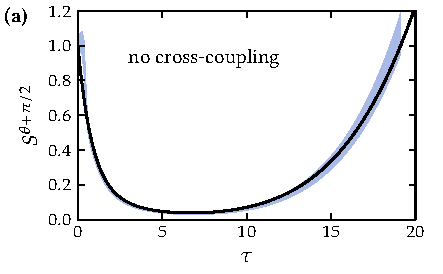
\includegraphics{figures_generated/exact/squeezing_nocc_100.pdf}%
    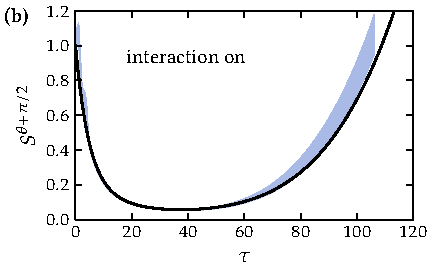
\includegraphics{figures_generated/exact/squeezing_cc_100.pdf}}

    \caption[Comparison of Wigner simulated spin squeezing with an exact method]{
    Comparison of the Wigner simulated time-dependent spin squeezing (blue bands; the width corresponds to the estimated sampling error) against the exact results (black lines), plotted on the logarithmic scale.
    Trajectories used: $2,000$.
    The plots correspond to \textbf{(a)} the case of no inter-component interaction ($\tilde{g}_{12} = 0$, $\tilde{g}_{11} = \tilde{g}_{22} = 1 / N$), and \textbf{(b)} strong inter-component interaction ($\tilde{g}_{ij} = a_{ij} / (a_{11} N)$, where $a_{11} = 100.4$, $a_{12} = 80.8$ and $a_{22} = 95.5$).}%endcaption

    \label{fig:exact:squeezing-comparison}
\end{figure}

The expectations above can be expressed in terms of creation and annihilation operators, and calculated either in Wigner representation using \thmref{mm-wigner:mm:moments}, or with the number state expansion using~\eqnref{exact:exact-a} and~\eqnref{exact:exact-f}.
The results for $S_{\theta+\pi/2}$ are plotted in~\figref{exact:squeezing-comparison}, using a low number of trajectories ($2,000$) for the truncated Wigner in order to make sampling errors more distinguishable.
The Wigner method shows good agreement with the exact results in the time range of interest; the growing sampling error can be reduced to a desirable extent by using more simulation trajectories.

\begin{figure}
    \centerline{%
    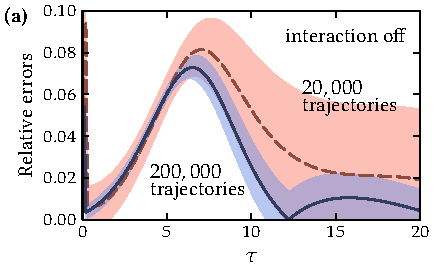
\includegraphics{figures_generated/exact/squeezing_nocc_err.pdf}%
    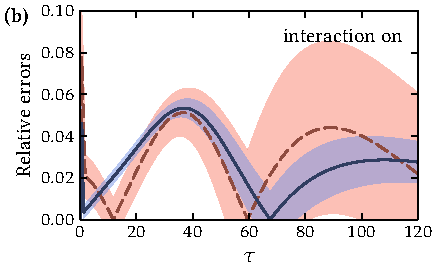
\includegraphics{figures_generated/exact/squeezing_cc_err.pdf}}

    \caption[Sampling and systematic errors in Wigner simulated spin squeezing]{
    Difference of the Wigner simulated spin squeezing $S_{\theta+\pi/2}$ and the exact results (lines) as compared to the sampling errors in Wigner simulations (bands), normalized by the exact results.
    The errors for $20,000$ trajectories (red dashed lines) and $200,000$ trajectories (blue solid lines) are plotted.
    The plots correspond to \textbf{(a)} the case of no inter-component interaction, and \textbf{(b)} strong inter-component interaction (the interaction coefficients are the same as in~\figref{exact:squeezing-comparison}).}%endcaption

    \label{fig:exact:squeezing-error-comparison}
\end{figure}

The relative (normalized on the corresponding results from the exact method) sampling and systematic errors of the Wigner method are plotted in~\figref{exact:squeezing-error-comparison}.
The Wigner results show a systematic error several times bigger than the corresponding sampling error in the first half of the time interval, which is a sign of the failing truncation approximation.
At other times, the difference with the exact results is within the sampling error range.
The large oscillations of the systematic error at the start of the simulation can be explained by accumulating uncertainties in the denominator of~\eqnref{exact:squeezing}.

\begin{figure}
    \centerline{%
    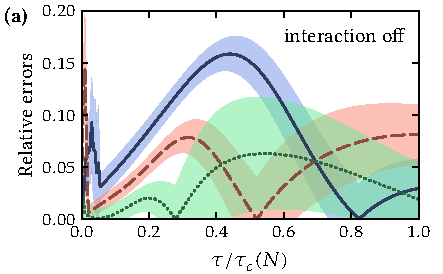
\includegraphics{figures_generated/exact/squeezing_nocc_N_err.pdf}%
    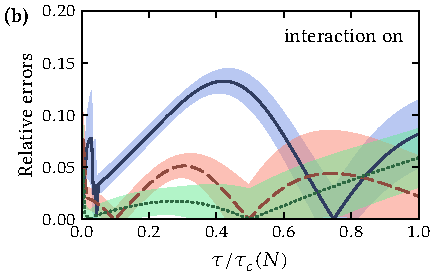
\includegraphics{figures_generated/exact/squeezing_cc_N_err.pdf}}

    \caption[Dependence of systematic errors in Wigner simulated spin squeezing on the particle number]{
    Difference of the Wigner simulated spin squeezing $S_{\theta+\pi/2}$ and the exact results (lines) as compared to the sampling errors in Wigner simulations (bands), normalized on the exact results.
    The errors for $N=20$ (blue solid lines), $N=200$ (red dashed lines) and $N=2,000$ (green dotted lines) with $200,000$ trajectories are plotted.
    The plots correspond to \textbf{(a)} the case of no inter-component interaction, and \textbf{(b)} strong inter-component interaction (the interaction coefficients are the same as in~\figref{exact:squeezing-comparison}).}%endcaption

    \label{fig:exact:squeezing-N-error-comparison}
\end{figure}

It is also interesting to look how the systematic error changes with the mode population (\figref{exact:squeezing-N-error-comparison}).
Since the time scale of the evolution varies with $N$, for this plot we normalized the time $\tau$ on the ``characteristic time'' $\tau_c(N)$, which corresponds to the time from the beginning of the evolution at which the squeezing $S_{\theta+\pi/2}$ rises back to $1$.
As expected, the larger is the population $N$, the smaller is the systematic error.
This indirectly confirms the truncation condition~\eqnref{wigner-bec:truncation:delta-condition}.

It must be emphasized that, while relative systematic errors are noticeable (about $5\%$ at the maximum), they correspond to the periods with low values of $S$ (see~\figref{exact:squeezing-comparison}).
Therefore, the absolute error is extremely low (of the order of tenths of decibel).
On the other hand, the technical noise in spin squeezing experiments can reach $10\un{dB}$~\cite{Riedel2010}.
This means that the systematic errors in the truncated Wigner method are far from being detectable by current technology.

Note that, while in this particular example the exact method gives more accurate results at comparable or lower computational cost, it becomes unapplicable as soon as one wants to include tunneling and nonlinear losses into the model, while the Wigner method continues to perform with the same efficiency~\cite{Opanchuk2012a}.

In conclusion, we have decisively shown that the truncated Wigner method gives accurate predictions for sophisticated compound observables (the squeezing~\eqnref{exact:squeezing} is calculated as a fourth order moment divided by a second order moment).
The system used in this chapter was a very simple one; for more complex systems it is possible to perform comparisons with the exact (in the limit of infinite simulation trajectories) positive-P phase-space method~\cite{Drummond1993,Chaturvedi2002,Dechoum2004}.
A detailed study of the validity of the truncated Wigner method was carried out by Sinatra \textit{et~al}~\cite{Sinatra2002}.
